The issue of providing anonymity to users is a complex problem, and although there are several systems claiming to offer anonymity, it is challenging to determine the level of anonymity provided by these systems. Serjantov et al. proposed a probability-based model to define the extent of anonymity provided by a system \cite{andreiInformation}. This model seeks to quantify the level of anonymity based on the probability of identifying the user who generated a particular message.

In a similar vein, David Chaum, while studying the security of Dining Cryptographers' networks, introduced the concept of an anonymity set \cite{dining}. The anonymity set is defined as the group of all possible participants in a network who could have sent a specific message, while all communication in the network is visible to an attacker. According to Chaum, the larger the anonymity set, the more difficult it becomes for an attacker to identify the sender of a message. Thus, the size of the anonymity set is an excellent indicator of the degree of anonymity provided by the network.

However, attacks in their literature review showed the probability of any subject sending or receiving a message is uniform and hence the size of the set is a good indicator of anonymity. However, in real-world scenarios, the probability of a subject sending or receiving a message is not uniform since an attacker can secure additional information and reduce the set size based on this information. For instance, in Figure \ref{fig:mix}, we see that if the attacker has the information that A sent a message to R then the attacker can immediately deduce the fact that S recieved a message from E. This is depsite the fact that the anonymity set for senders of S is \{A, B, C, D, E\}. 

\begin{figure}[H]
\centering
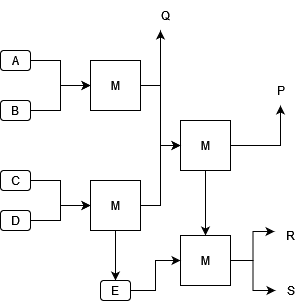
\includegraphics[width=0.6\textwidth]{images/mix.png}
\caption{An attack in mix networks. Here, M are the mixes and A, B, C, D, E are the senders.}
\label{fig:mix}
\end{figure}

Following this review we come to a conlcusion that we need a better metric to determine the quality of anonymity offered to the users. Serjantov et al. introduce entropy to describe quality of anonymity \cite{andreiInformation}. Entropy is a measure of the uncertainty of a random variable \cite{shannon}. In this scneario, the attacker has a probability distribuition, $P$, over the set of all participants with regards to them sending or receiving a message. They now define the effective size of the probability distribuition to be equal to the entropy of the distribuition: 
\begin{equation}
    \label{eq:entropy}
    S = -\sum_{u \in \Psi} p_u \log_2 p_u
\end{equation}
Here, $p_u$ is $P(u, r)$, $\Psi$ is the set of all participants and $r \in$ \{sender, recepient\}. This can also be interpreted as the number of bits of additional information required to identify a user of a particular message.



